%\documentclass[10pt,a4paper]{article}
\documentclass[12pt,a4paper]{article}
\usepackage{graphicx,amsmath}
%\usepackage{subfigure}
\usepackage{float}
\usepackage[german]{babel}
\usepackage[utf8]{inputenc}
\setcounter{secnumdepth}{4}
\usepackage[top=2cm, bottom=2.5cm, left=3cm, right=3cm]{geometry}
\begin{document}


%\title{Bachelorarbeit}
%\author{Richard Kullmann}
%\date{02.06.2017}

\thispagestyle{empty}
%\setcounter{page}{2}
\newpage
\tableofcontents
\thispagestyle{empty}
\newpage
\pagenumbering{arabic}

\section{Fano-Faktor im Neuronenmodell}
In dem Bereich des Maximums wurden noch ein paar Rechnungen durchgeführt, um die Rauschintensität des Maximums etwas besser einzugrenzen. Dabei ergaben sich folgende Bilder:
\begin{figure}[H]
	\centering
	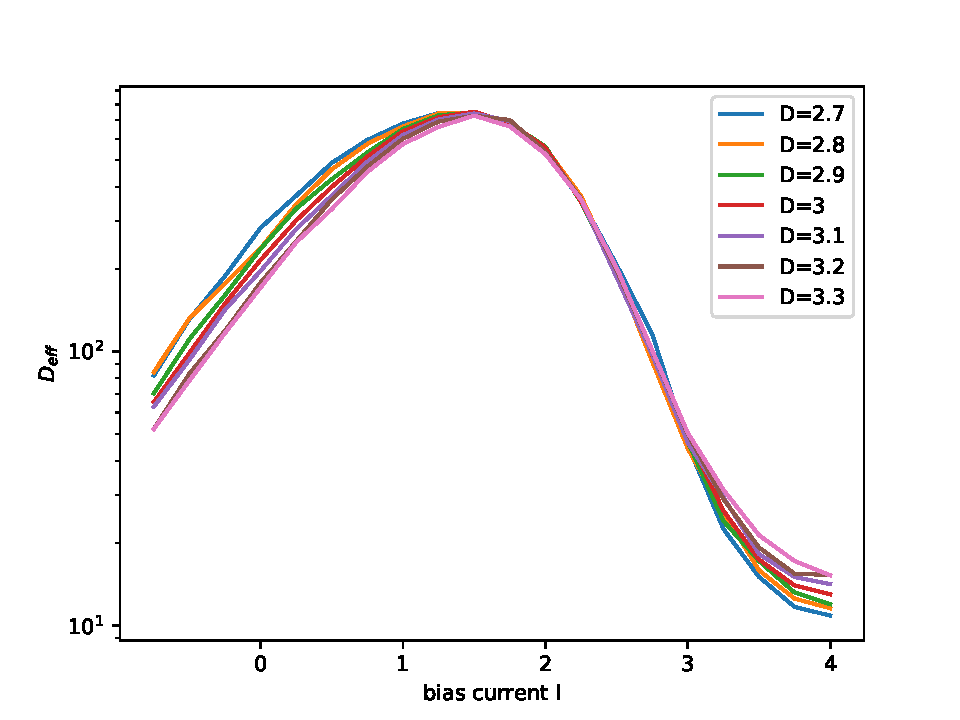
\includegraphics[scale=0.9]{dneurpmax.pdf} 
	\caption{Diffusionskoeffizienten für verschiedene Rauschintensitäten nahe des Maximums}
	\label{dnpmax}
\end{figure} 
\begin{figure}[H]
	\centering
	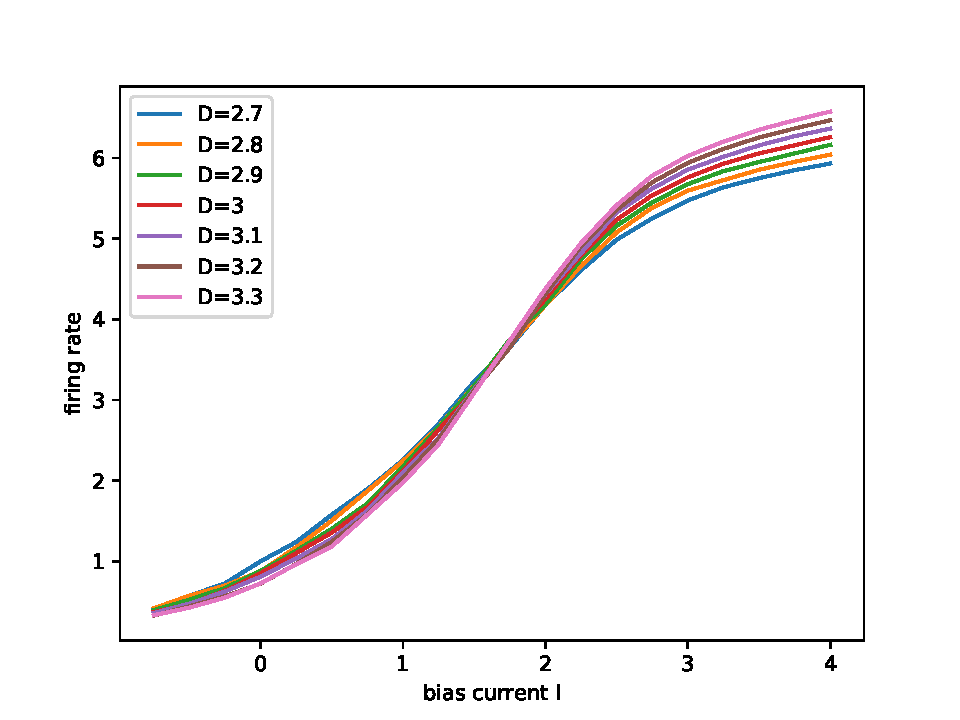
\includegraphics[scale=0.9]{gneurpmax.pdf} 
	\caption{Feuerraten für verschiedene Rauschintensitäten nahe des Maximums}
	\label{gnpmax}
\end{figure} 
\begin{figure}[H]
	\centering
	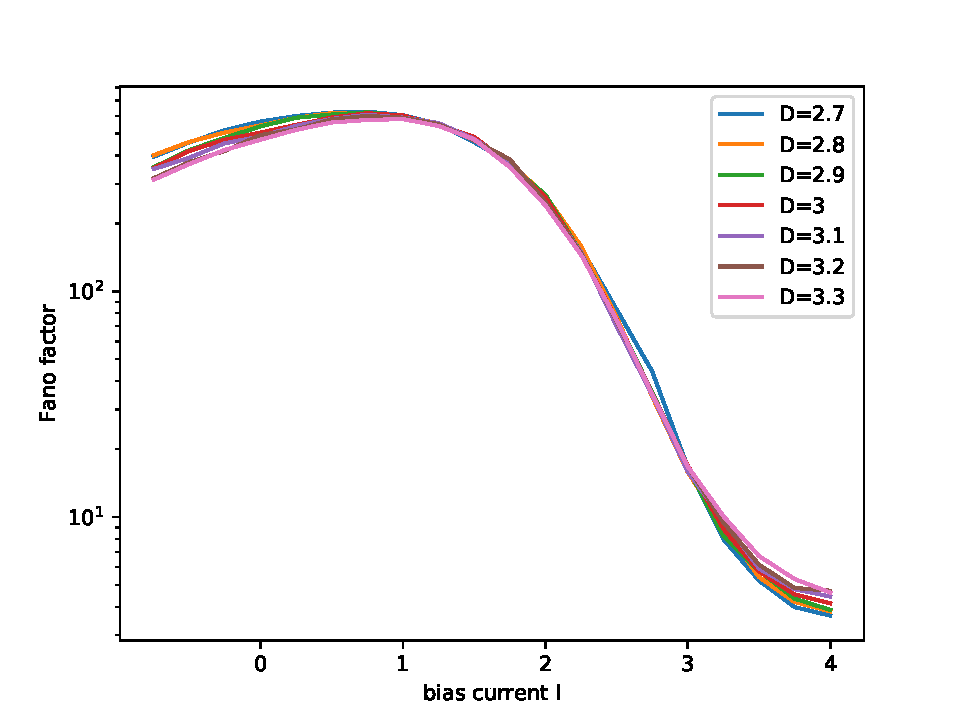
\includegraphics[scale=0.9]{fneurpmax.pdf} 
	\caption{Fano-Faktoren für verschiedene Rauschintensitäten nahe des Maximums}
	\label{fnpmax}
\end{figure} 
Eine Vergrößerung des Bildausschnitts zeigt, dass das Maximum des Diffusionskoeffizienten tatsächlich bei genau 3 zu finden ist. Der Fano-Faktor erreicht sein Maximum bei einem anderen Wert, der aus den bisherigen Messungen aber noch nicht ersichtlich wird:

\begin{figure}[H]
	\centering
	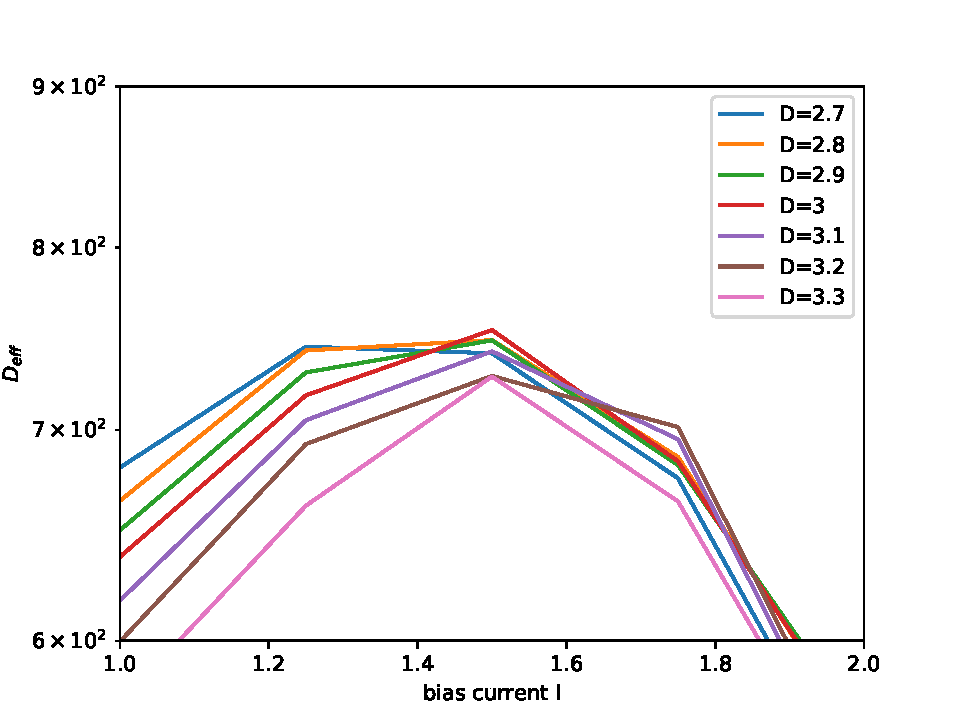
\includegraphics[scale=0.9]{dneurpmaxclose.pdf} 
	\caption{Diffusionskoeffizienten für verschiedene Rauschintensitäten nahe des Maximums}
	\label{dnpmaxcl}
\end{figure} 

\begin{figure}[H]
	\centering
	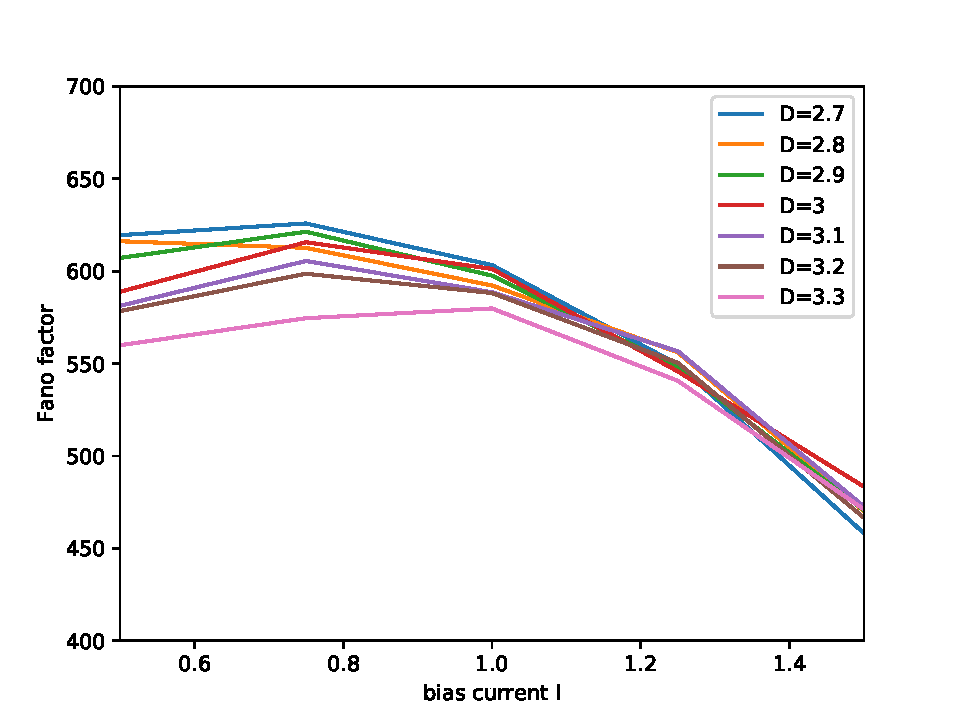
\includegraphics[scale=0.9]{fneurpmaxclose.pdf} 
	\caption{Fano-Faktoren für verschiedene Rauschintensitäten nahe des Maximums}
	\label{fnpmaxcl}
\end{figure} 
Damit wurde die Rauschintensität beim Maximum mit einem Fehler von unter 5\% berechnet, was vorerst genügt. 
\section{Parameter im Neuronenmodell}
Da das Neuronenmodell einige Ähnlichkeiten mit dem mechanischen Modell aufweist, ist zu vermuten, dass andere Parameter auch zu einem anderen Verhalten des Neuronenmodells führen. \\
Hier ist noch einmal das betrachtete Modell:

\begin{align*}
C\dot{V} &= I - g_L(V-E_L) - g_{Na}m_{\infty}(V)(V-E_{Na}) - g_Kn(V-E_K)+\sqrt{2D}\xi(t)\\
\dot{n} &= (n_{\infty}(V)-n)/\tau(V)
\end{align*}
Mit
\begin{align*}
f_{\infty}(V) = \frac{1}{1+\exp\{(V_{1/2}-V)/k\}}
\end{align*}
und den folgenden Parametern:\\
$C=1$ , $g_L=8$ , $E_L=-80$ , $g_{Na}=20$ , $E_{Na}=60$ , $g_K=9$ , $E_K=-90$.
\begin{align*}
\intertext{Instantaner $Na^+$-Strom:} &k_m=15 , V_{1/2,m}=-20. 
\\
\intertext{$K^+$-Strom:} &k_n=5 , V_{1/2,n}=-25 , \tau(V)=0.152.
\end{align*}
Als erstes wurden nun die Zeitkonstanten $k_m$,$k_n$ und $\tau(V)$ bei $D=3$ und $I=1.5$ variiert:
\begin{figure}[H]
	\centering
	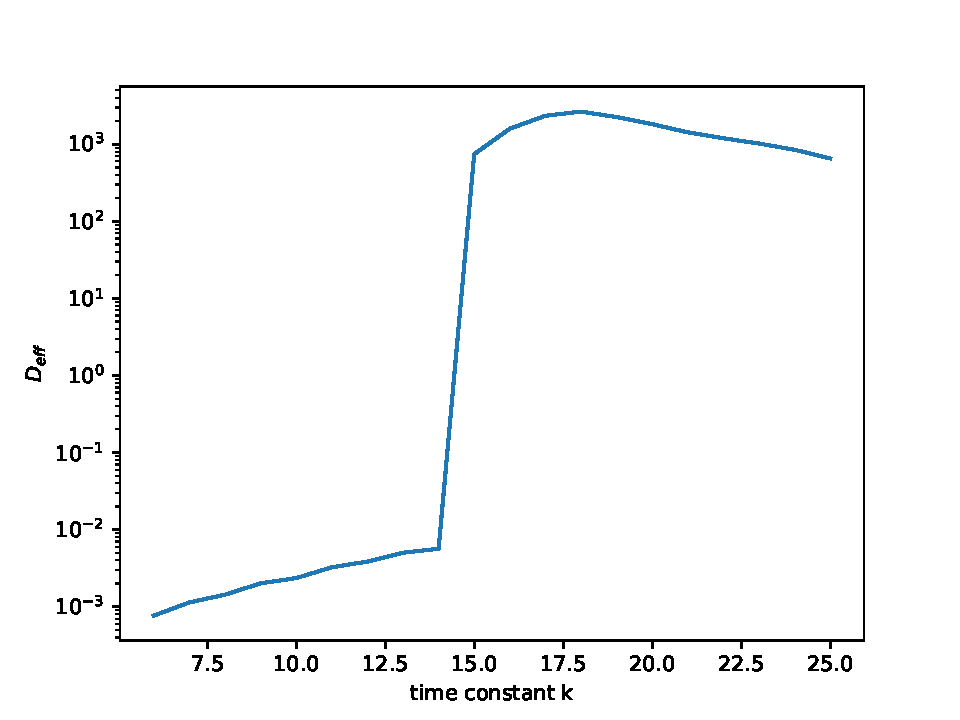
\includegraphics[scale=0.9]{dneurkvar.pdf} 
	\caption{Variation von $k_m$}
	\label{kmvar}
\end{figure} 
\begin{figure}[H]
	\centering
	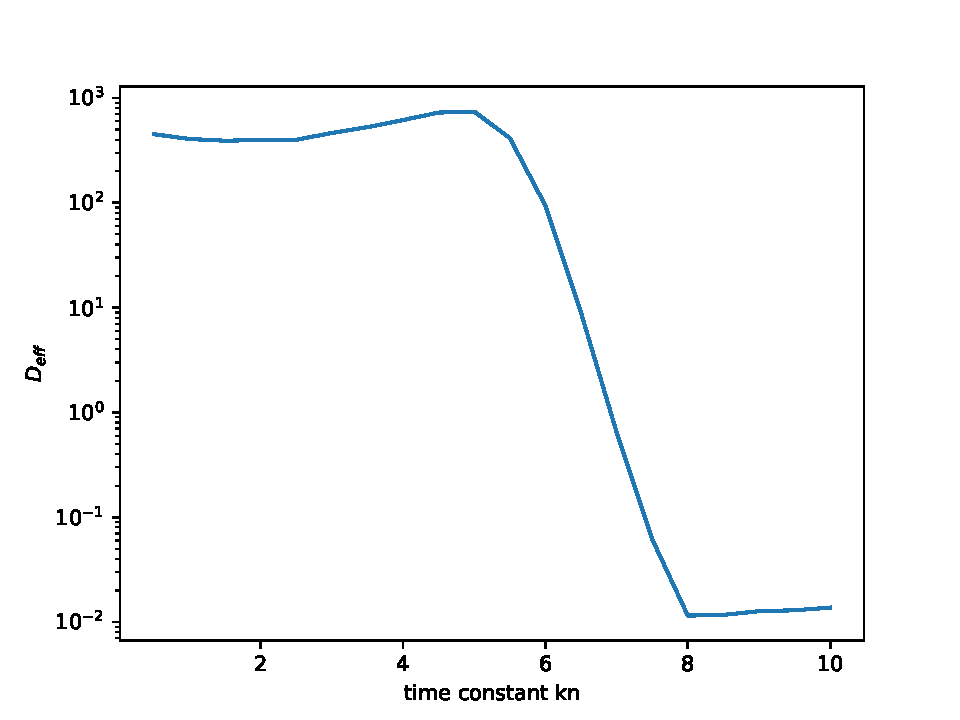
\includegraphics[scale=0.9]{dneurknnvar.pdf} 
	\caption{Variation von $k_n$}
	\label{knvar}
\end{figure} 
\begin{figure}[H]
	\centering
	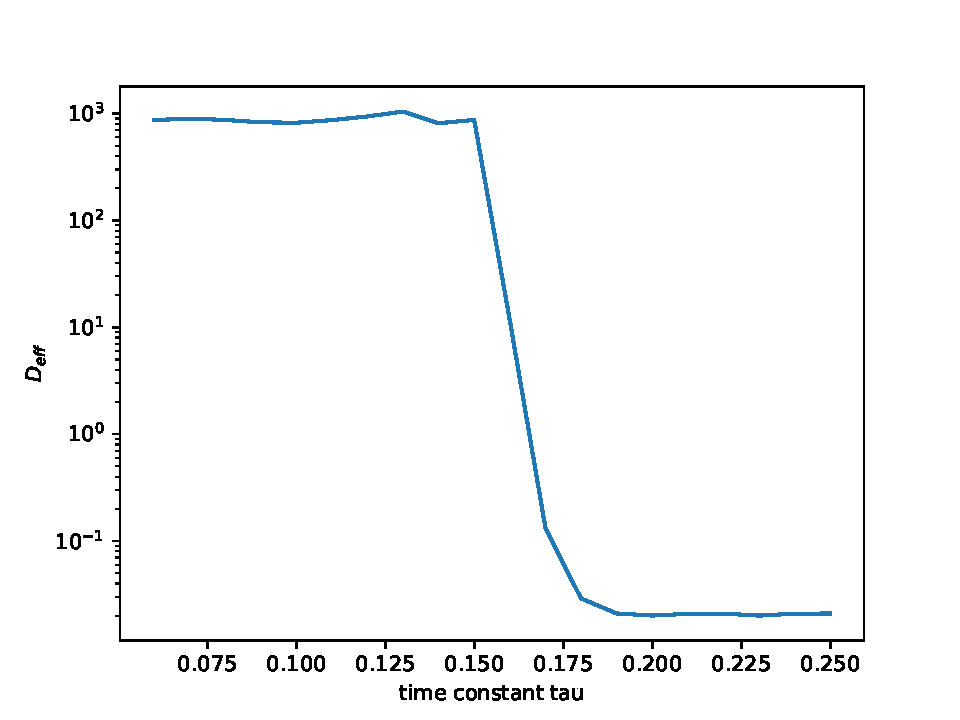
\includegraphics[scale=0.9]{dneurtvar.pdf} 
	\caption{Variation von $\tau(V)$}
	\label{tvar}
\end{figure} 
Dann wurden $g_K$ und $g_L$ verändert:
\begin{figure}[H]
	\centering
	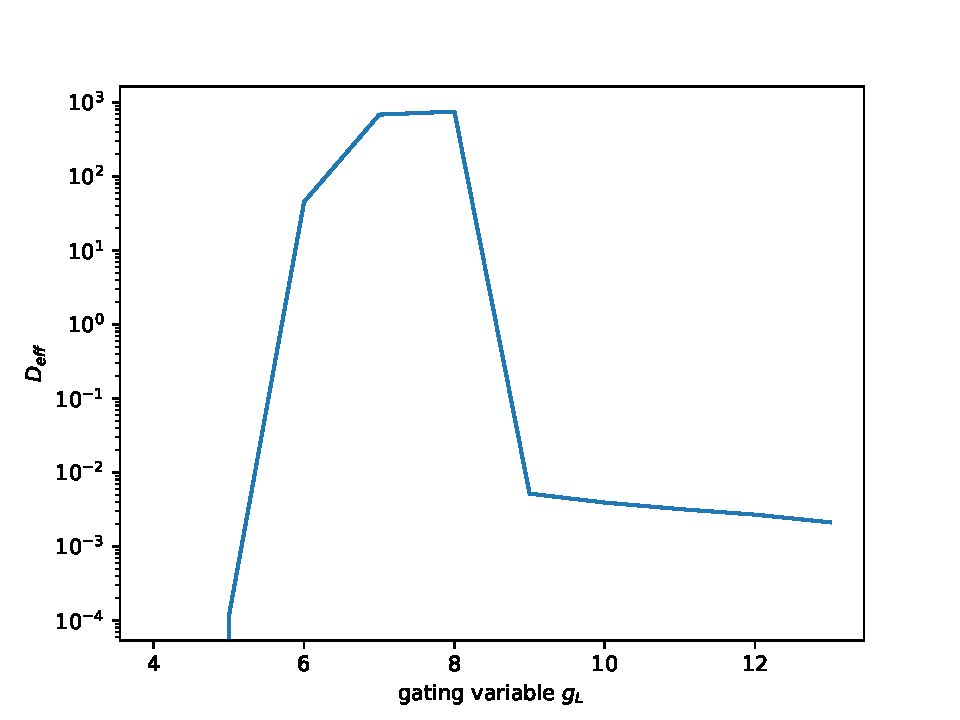
\includegraphics[scale=0.9]{dneurglvar.pdf} 
	\caption{Variation von $g_L$}
	\label{glvar}
\end{figure} 
\begin{figure}[H]
	\centering
	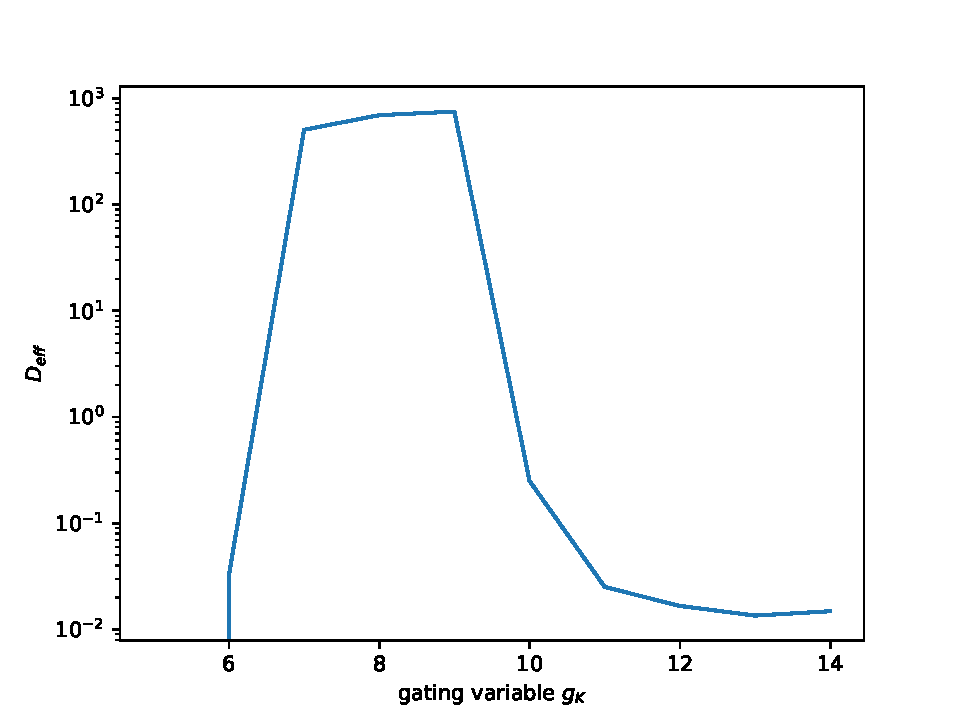
\includegraphics[scale=0.9]{dneurgkvar.pdf} 
	\caption{Variation von $g_K$}
	\label{gkvar}
\end{figure} 
Es ist zu erkennen, dass Veränderungen der Größen höchstens eine starke Verringerung des Diffusionskoeffizienten bewirken können, aber nicht das erwartete exponentielle Wachstum.\\
Weiteres Vorgehen: Überprüfung von anderen Neuronenmodellen  auf Giant Diffusion, z.B. $I_{Na,t}$-oder $I_h+I_{Kir}$-Modell. Wichtig ist hierbei, dass qualitativ verschiedene Modelle gefunden werden, da sonst kein neues Verhalten erwartet werden darf.
\section{mechanisches Modell}
Für die verschiedenen Temperaturen wurde zunächst die Konvergenz des gemittelten Diffusionskoeffizienten untersucht:
\begin{figure}[H]
	\centering
	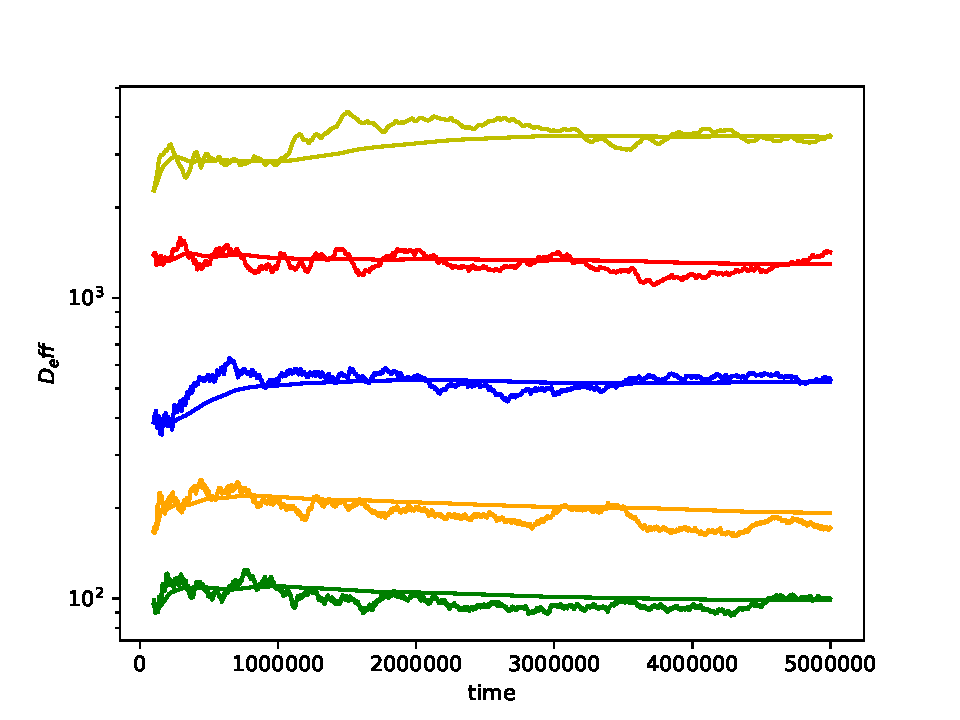
\includegraphics[scale=0.9]{dmechav.pdf} 
	\caption{Vergleich von gemittelten und tatsächlichen Diffusionskoeffizienten; der oberste Graph entspricht $kT=0.033$, der unterste entspricht $kT=0.094$}
	\label{dav}
\end{figure} 
Davon ausgehend wurde eine Simulationszeit von $T_{max}=5\cdot 10^6$ gewählt, und ab $T_{eq}=2\cdot 10^6$ wurde gemittelt:
 
\begin{figure}[H]
	\centering
	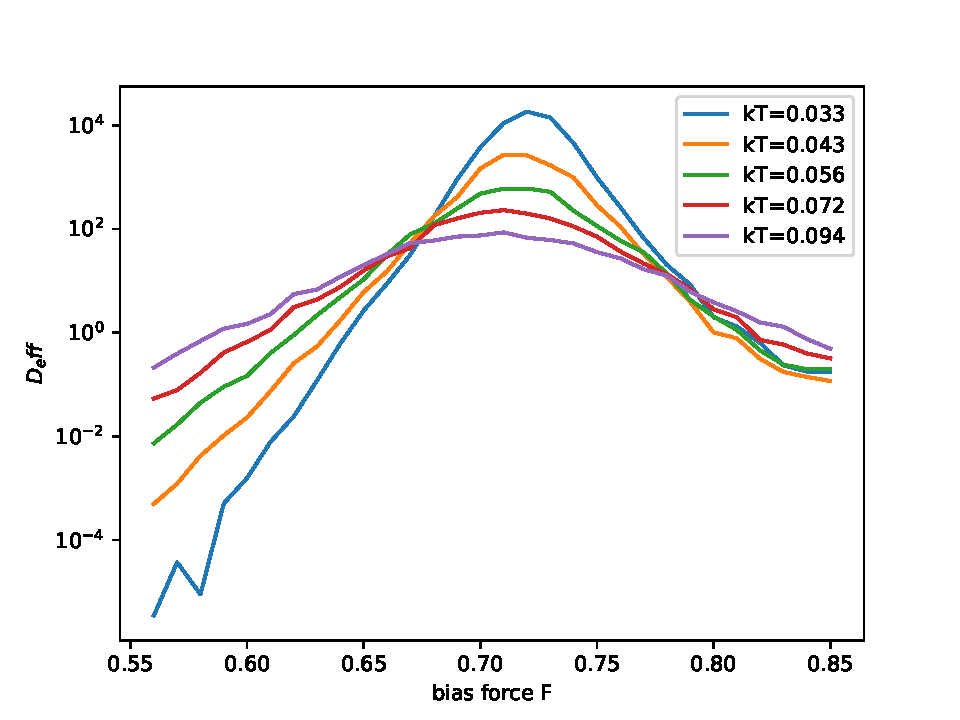
\includegraphics[scale=0.9]{dmechex.pdf} 
	\caption{Diffusionskoeffizienten für längere Laufzeiten}
	\label{dex}
\end{figure} 
\begin{figure}[H]
	\centering
	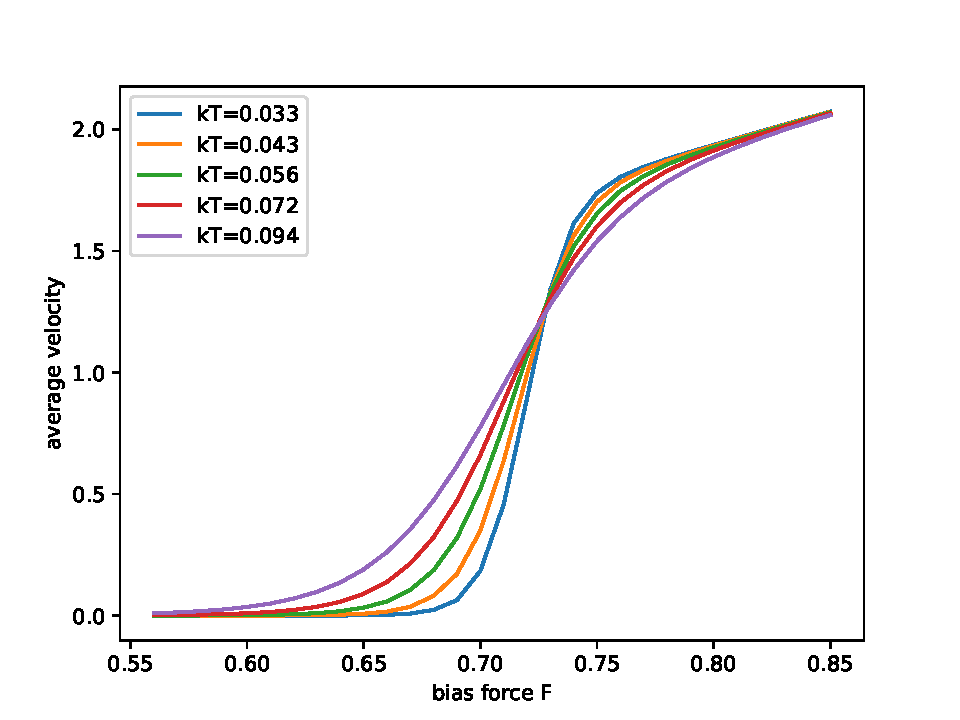
\includegraphics[scale=0.9]{gmechex.pdf} 
	\caption{mittlere Geschwindigkeiten für mittlere Laufzeiten}
	\label{gex}
\end{figure} 
\begin{figure}[H]
	\centering
	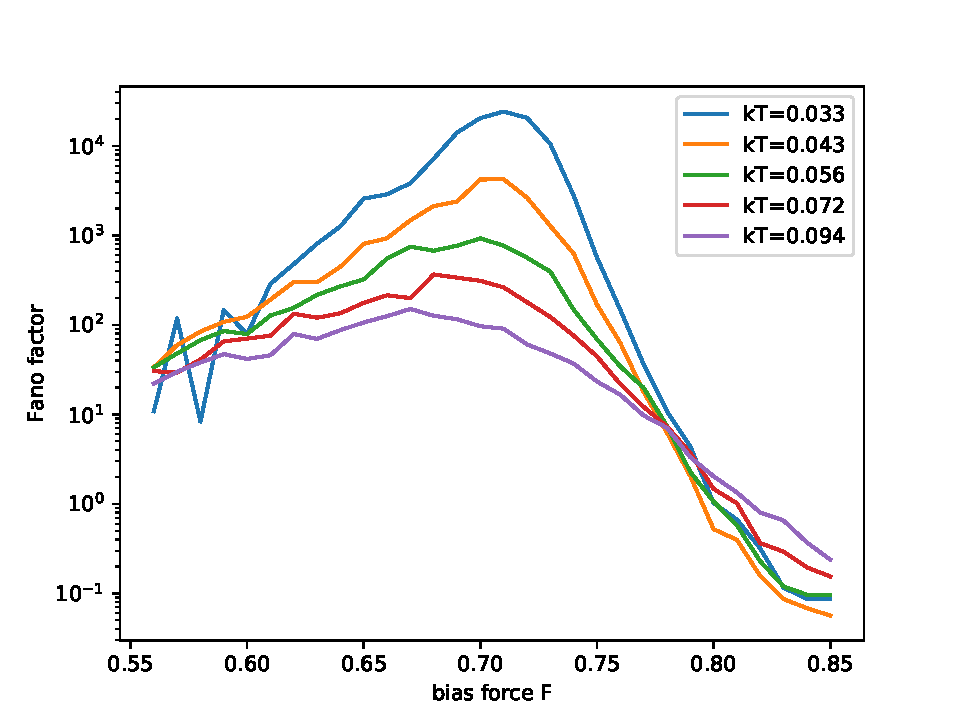
\includegraphics[scale=0.9]{fmechex.pdf} 
	\caption{Fano-Faktoren für längere Laufzeiten}
	\label{fex}
\end{figure} 
Wie auch vorher schon passt die Kurve mit $kT=0.033$ noch nicht zu den anderen, was den rechten Schnittpunkt angeht. Diese Kurve wird also noch einmal mit höherer Genauigkeit berechnet. Damit wird die Betrachtung des mechanischen Modells dann jedenfalls vorerst auf Eis gelegt. 
\end{document}

